\subsection{Collaborative evidence collection}

Teams responded positively on the evidence collection capability. The annotation tool enables them to mark key information as they read through and documents and model data objects for analysis simultaneously. 

\begin{quote}
	I think the tool is extremely helpful for collaborating on highlighting key evidence. It is hard to remember what you were thinking when reading a piece of evidence, but with CAnalytics you can annotate it while you read to remember what you were thinking. (P68)
\end{quote}

\begin{figure}
	\centering
	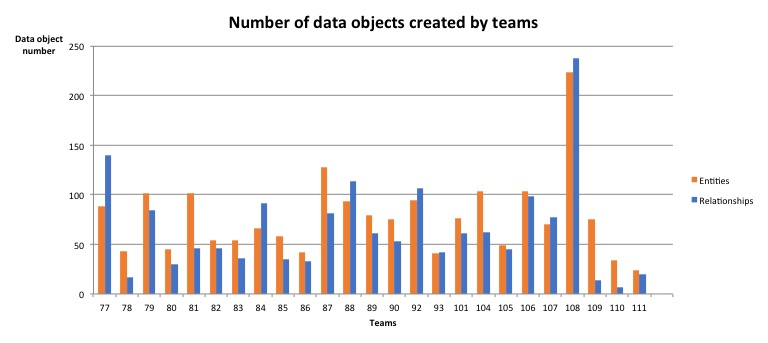
\includegraphics[height=1.5in]{img/user_created_objects}
	\caption{The number of entities and relationships that the groups created.}
	\label{fig:user_created_objects}
\end{figure}

The 25 teams created 1919 entities and 1636 relationships in total (Figure~\ref{fig:user_created_objects}). The number of entities each team created ranges from 24 to 223 (M=76, SD=40.2), and the relationships ranged from 7 to 237 (M=65, SD=49.1). One reason causing the wide variety is the usage of CAnalytics in the task (e.g. Team 111 did not use much of CAnalytics as other teams did), but the major reason is the different strategies teams took in approaching the task. Teams adopted different levels of granularity when collecting evidence. Figure~\ref{fig:network_example} shows two exemplar node-link graphs that illustrate the evidence two teams collected. Team 108 modeled suspect's every single action as an event, in an attempt to discover connections between robbery cases by examining similarities and dissimilarities in suspects' behavior patterns. In contrast, Team 107 only extracted high-level entities and modeled a whole robbery case as an event, resulting in many fewer data objects. The graph provides an overview of the seven cases and relationships among suspects. Neither strategy is better than the other, because they offer different insights and could be utilized in different stages of analysis. Two questions must be addressed here: 1. how should team members coordinate themselves to keep consistent with information granularity when collecting evidence; 2. how can the system provide a proper view for multiple levels of evidence granularity? The graph by Team 108 is obviously too noisy to provide insight. 

\begin{figure}
\centering
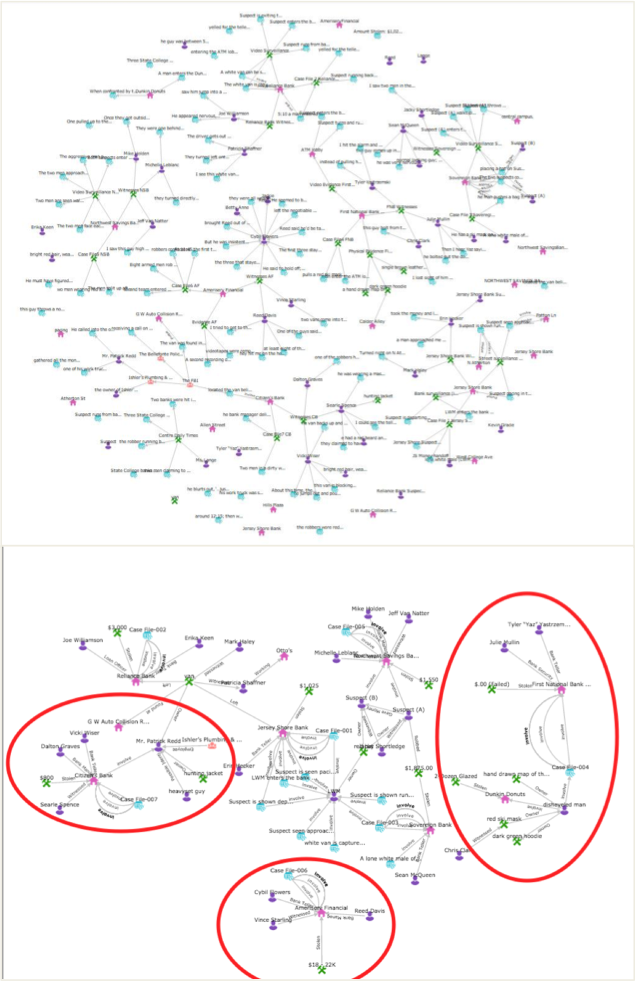
\includegraphics[width=0.7\linewidth]{img/network_example}
\caption{Two node-link graphs created by student analysts. The top one (by Team 108) contains a large number of nodes and links, describing every single action of suspected robbers. The bottom one (by Team 107) contains fewer nodes and links, describing only high-level events}
\label{fig:network_example}
\end{figure}

\hl{categorize entities inconsistently}
Another primary collaborative breakdown during evidence collection is inconsistency of data modeling. For example, some named entities could be modeled as different categories of data objects (e.g. a bank can be treated as an organization or a location). While such inconsistencies are superficial, they could lead to team confusion and misinterpretations. Such information serves as foundation for evidence schematization from which a team draws conclusion. 

